\chapter{Mise en pratique future}
\label{chap:future-works}
Dans nos analyses au chapitre \ref{chap:analyse}, nous montrons le besoin d'effectuer des tests comparatifs pour corriger les biais trouvés sur les résultats observés. Nous montrons aussi la nécessité de mettre en place une méthodologie de comparaison équitable entre la FSOD et le TL afin d'expérimenter et comprendre les avantages et les inconvénients des deux approches. Dans ce chapitre, nous décrivons les travaux que nous ferons pour la suite du projet, dont le but sera de répondre aux besoins évoqués.

% Base de comparaison des
\section{Mise au point d'une base de comparaison}
Pour notre travail de comparaison, nous décidons de sélectionner les algorithmes de détection dont le code est fourni par les rédacteurs des articles trouvés pendant notre bibliographie. Cela nous permet de nous concentrer sur l'analyse et la comparaison des résultats fournis par ces détecteurs. Dans le cas où une implémentation venait à manquer pour un détecteur particulièrement intéressant, nous essayerons de la fournir.

\subsection{Comparaison "intra-approche"}
Pour obtenir une analyse pertinente des résultats des détecteurs d'une même approche (FSOD ou TL), nous devons effectuer des tests sur les mêmes tâches et les mêmes données, afin d'être sûr de limiter les biais de comparaisons. Cela se traduit, de manière générale, par l'utilisation des mêmes datasets et la définition du même problème de détection à résoudre. Spécifiquement, pour la FSOD, il faut également assurer une sélection des tâches $N$-way $K$-shot équitable pour éviter le biais de la difficulté des images variable qui influence la performance. % TODO ?

\subsection{Comparaison "inter-approches"}
Notre travail consistera désormais à tester certaines méthodes de transfer learning et de few-shot object detection. Dans ce cas, la difficulté est de comparer efficacement les deux approches au vu de la métrique intrinsèque à chacune des approches. Nous nous effectuerons des tests sur des bases de données identiques. Nous essayerons de mettre au point une méthodologie qui permet de réaliser une comparaison équitable, c'est-à-dire qui n'avantage pas l'apprentissage ou la détection d'un détecteur d'une approche par rapport à l'autre.

%Le transfer learning étant vaste et le few-shot en étant un cas particulier, il faut nous concentrer sur un cas particulier du TL. Un cas intéressant est le multi-tasking learning permettant de faire l'apprentissage de plusieurs taches en simultanée. La base de données d'image est ici fourni en plus du code.

%De même nous pourrons tester un réseau de Deep transfère Learning avec les JAN (joint Adaptation Networks) qui va permettre de travailler sur des base de données plus communes du type ImageNet ou Office-31.

\section{Interface de simulation de détections}
En parallèle de notre travail d'analyse, nous proposerons une vue de notre travail au moyen d'une interface permettant de simuler des détections avec les algorithmes que nous avons utilisé dans notre travail de comparaison. Le but de cette interface est de fournir à un utilisateur une vue concrète des performances des détecteurs en transfer learning et en few-shot object detection. La figure \ref{fig:UML_INTERFACE} illustre les fonctionnalités de l'interface.
\begin{figure}[!h]
\centering
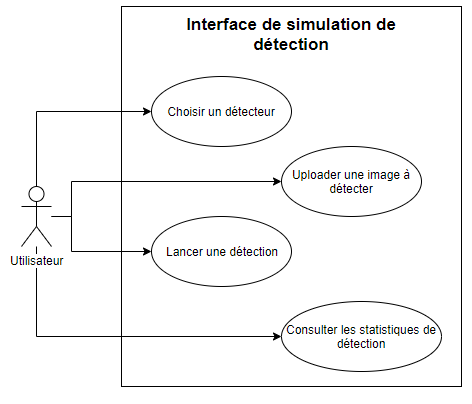
\includegraphics[scale=0.5]{img/UML_INTERFACE.PNG}
\caption{Diagramme UML présentant les fonctionnalités de l'interface de simulation de détections à réaliser.}
\label{fig:UML_INTERFACE}
\end{figure}

%Ensuite nous proposerons une vue de notre travail avec une démonstration qui permettra de voir des comparaisons de plusieurs réseaux. Nous espérons ainsi laisser l'utilisateur pouvoir choisir entre des réseaux non entraînés avec des méthodes de TL et des réseaux de TL et lui laisser voir que les méthodes de TL fonctionnent mieux sur des vidéos contenants plusieurs objets.

%De même afin que l'utilisateur puisse constater ça de lui-même, l'utilisateur pourrait tester le réseau grâce à la webcam du PC de démo.